\documentclass{beamer}

\usepackage{setspace}

% config du thgeme metropolis
\usetheme[progressbar=frametitle,block=fill, titleformat=smallcaps,sectionpage=progressbar,]{metropolis}



\title{Analyse en Composantes Principales}
\subtitle{}
\date{2021-2022}
\author{Paul Chapron \textsuperscript{1} \& Yann Ménéroux \textsuperscript{1}}
\institute{ \textsuperscript{1}IGN-ENSG-UGE}



%definition de la couleur du texte dans la balise \alert{}
\definecolor{vertIGN}{HTML}{96C31E} % vert IGN %vrai valeur #97BE0D
\setbeamercolor{alerted text}{fg=vertIGN}

\definecolor{grisIGN}{HTML}{22292F} % Gris IGN tiré vers le noir 
\setbeamercolor{background canvas}{bg=grisIGN}




% code pour placer le log ENSG dans le bandeau de titre 
\makeatletter
\setbeamertemplate{frametitle}{%
  \nointerlineskip%
  \begin{beamercolorbox}[%
      wd=\paperwidth,%
      sep=0pt,%
      leftskip=\metropolis@frametitle@padding,%
      rightskip=\metropolis@frametitle@padding,%
    ]{frametitle}%
  \metropolis@frametitlestrut@start%
  \insertframetitle%
  \nolinebreak%
  \metropolis@frametitlestrut@end%
  \hfill
  \raisebox{-0.6ex}{
\includegraphics[height=4ex,keepaspectratio]{img/logoENSG_small.jpg}}
  \end{beamercolorbox}%
}
\makeatother




% logo ENSG première page 
\titlegraphic{\vspace{4cm}\flushright
\includegraphics[width=2cm,height=2cm]{img/logoENSG_big.png}} 



\begin{document}
\metroset{background=dark} % change background theme according to manual
\maketitle	

\section{Introduction} 

\begin{frame}{Dans les cours précédents ... }


Techniques pour quantifier la liaison entre \alert{deux} variables (quali ou quanti). 

\begin{itemize}
\item corrélation
\item régression linéaire
\item $\chi^2$  (test d'indépendance)
\item visualisation adéquate 
\end{itemize}

\end{frame}


\begin{frame}{Motivation}


La plupart des phénomènes intéressants (sociaux, spatiaux) sont \alert{multi-factoriels}. Les données disponibles pour les décrire sont :

\begin{itemize}
	\item partiellement \alert{redondantes}  :   e.g. revenu et profession
	\item intrinsèquement \alert{corrélées} : e.g. revenu et taille du logement
	\item parfois des proportions (somme à 1 ou 100\%)
\end{itemize}
\end{frame}

\begin{frame}{Quoi et Comment}
L'analyse \alert{factorielle}  cherche à réduire la \alert{colinéarité} et le \alert{nombre de dimensions} (=variables) qui décrivent une population ... 

\medskip \medskip

... en proposant de nouvelles variables \alert{composites décorrélées}.
\end{frame}


\begin{frame}{Une population}
\centering
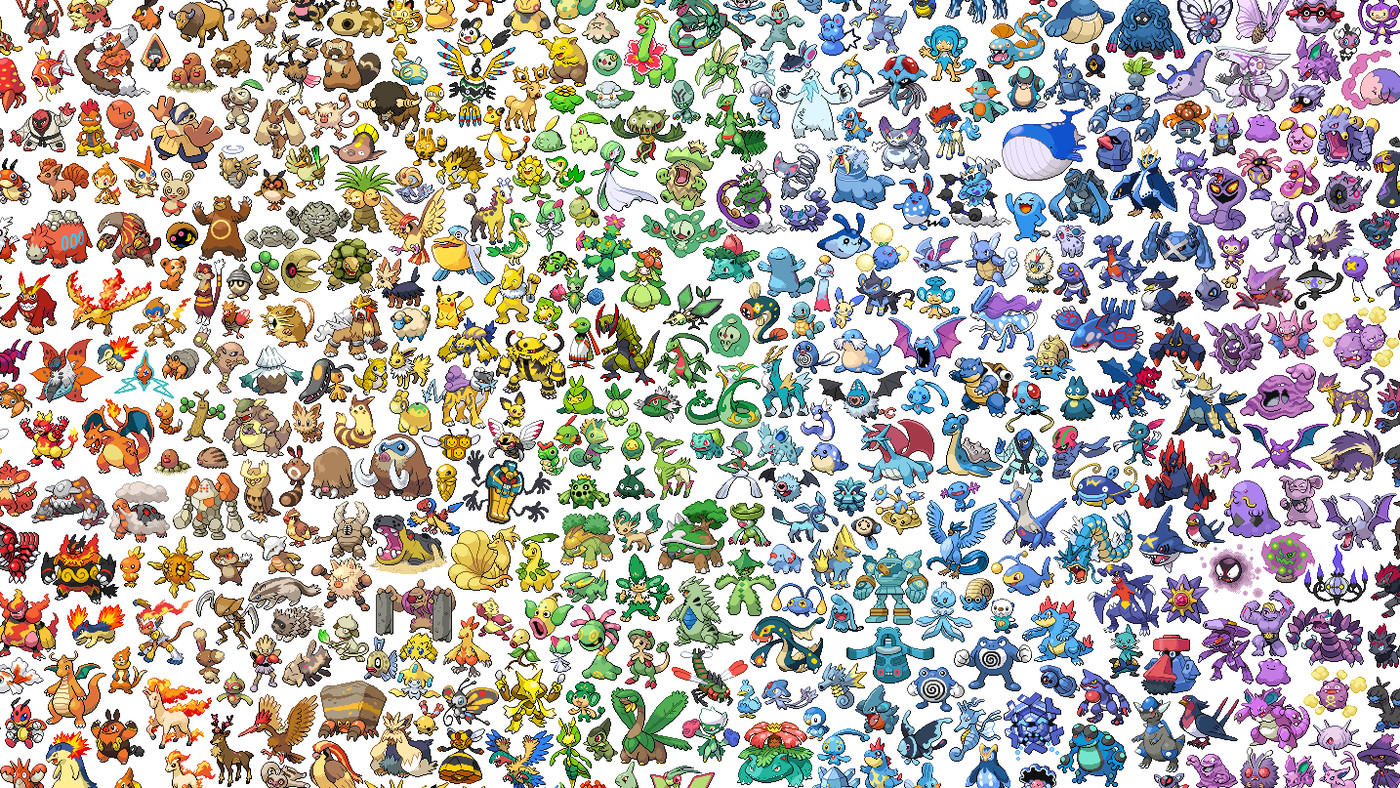
\includegraphics[width=\textwidth,keepaspectratio]{img/pokemons.jpeg}
\end{frame}

\begin{frame}{Plusieurs dimensions}
\centering
\begin{itemize}
	\item Nom e.g. "Pikachu"
	\item Type 1 $\in\{Grass,\ Fire,\ Water,\ Bug, \dots \}$
	\item Type 2 idem
	\item HP : numérique 
	\item Attack : numérique 
	\item Defense : numérique 
	\item Speed : numérique 
	\item Special Attack :numérique 
	\item Special Defense  : numérique
	\item Generation : facteur $\in \{1,2,3,4,5,6\}$
	\item Legendary : booléen
\end{itemize}

\end{frame}


\begin{frame}{Dimensions "composites"}


Existe-t-il des combinaisons qui \alert{résument bien} les caractéristiques des pokemons ? (moins de six!)

\medskip \medskip

Comment les constituer ? 

\medskip \medskip

i.e. comment \alert{combiner} les six variables numériques pour bien \alert{expliquer leur variation} au sein de la population ? 



\end{frame}

\begin{frame}{Attack vs. Defense}
\centering
\includegraphics[width=\textwidth,keepaspectratio]{img/Attack_Defense.png}
\end{frame}


\begin{frame}{Speed vs. HP}
\centering
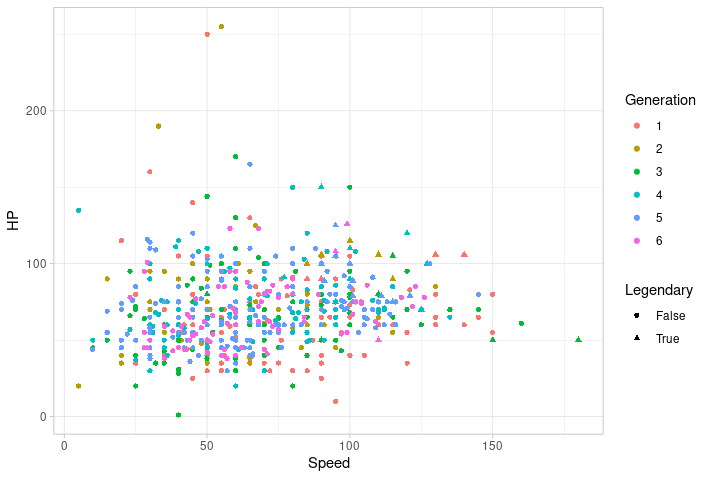
\includegraphics[width=\textwidth,keepaspectratio]{img/Speed_HP.png}
\end{frame}




\section{L'inertie}


\begin{frame}{L'inertie}
L'inertie est l'équivalent \alert{multi-dimensionnel} de la \alert{variance} d'une variable.


C'est une notion centrale de l'ACP.


$$I= \frac{1}{n}\sum_{i=1}^n d^2(x_i,g)$$

Avec 
\begin{itemize}
\item $n$ la taille de la population 
\item $x_i$ la valeur de la variable de l'individu $i$ 
\item $g$ le point moyen 
\item $d(x,y)$ une distance, souvent euclidienne : $(x_i-g_i)^2$ 
\end{itemize}
\end{frame}


\begin{frame}{L'inertie}

L'inertie quantifie la \alert{dispersion} du nuage de points

L'inertie est la "moyenne du carré des distances", ou encore la \alert{somme des variances} des variables

Inertie faible $\implies$ peu de variété dans les variables, individus semblables, faible quantité d'information
\end{frame}


\begin{frame}{L'inertie en 1D}


Soit une population $P$ de $n$ individus décrits par une variable $X$

l'inertie de la population est la \alert{variance} de $X$ : 

$$I= \frac{1}{n}\sum_{i=1}^n (x_i-\bar{x})^2$$

Le point moyen a pour "coordonnées" $\bar{x}$

\end{frame}


\begin{frame}{L'inertie en 2D}


Soient $X$ et $Y$ deux variables qui décrivent des individus $p_i$ de la population $P$, et $g=(x_g,y_g)$ le point moyen de cette population, de coordonnées $x_g=\bar{x}$ et $y_g=\bar{y}$.


L'inertie de $P$ est :  $$I= \frac{1}{n}\sum_{i=1}^n (x_i-x_g)^2 + (y_i-y_g)^2$$

On reconnaît une somme de variances : $I=var(X)+var(Y)$

\end{frame}


\begin{frame}{L'inertie en nD}

Soient  $v$ variables , notées $X^{(k)}, k \in \{1,\dots,v\}$ qui décrivent les individus d'une population $P$, le point moyen de $P$ est noté $g$.

L'inertie de $P$ est :  $$I= \frac{1}{n}\sum_{k=1}^v\sum_{i=1}^n (x_i^{(k)}-x^{(k)}_g)^2$$

on reconnaît $$I= \sum_{k=1}^v var(X^{(k)})$$

\end{frame}



\section{Espaces, vecteurs, axes, variables}


\begin{frame}{Individus dans l'espace d'origine}
L'ACP considère une population statistique décrite par plusieurs variables (continues).


Ces variables définissent un \alert{espace vectoriel} , qu'on va appeler l'espace d'\alert{origine}: 
\begin{itemize}
	\item un individu $i$ est un \alert{vecteur}
	\item la valeur de ses variables sont les \alert{coordonnées} du vecteur dans cet espace. 
	\item chaque variable est une \alert{dimension} de cet espace. elle définit un \alert{axe} de l'espace. (cf. axe des $x$ dans un repère orthonormé)
\end{itemize}

Les variables étant potentiellement \alert{corrélées}, les axes de l'espace de départ ne sont pas toujours (presque jamais) orthogonaux ! 


\end{frame}


\begin{frame}{Individus dans l'espace d'origine}

Les individus sont des vecteurs dans l'espace des variables 


\medskip mais également \medskip

Les variables sont des vecteurs dans l'espace des individus 


\end{frame}





\begin{frame}{Explicitation de l'ACP}


L'ACP consiste à trouver de  \alert{nouveaux axes orthogonaux entre eux}, qui capturent le \alert{plus d'inertie possible} de la population $P$.


Ces axes définiront un nouvel espace : l'\alert{espace d'arrivée}


On trouve ces axes en combinant (linéairement), les variables de la population $P$, par exemple :

$$ axe_1 = \alpha X + \beta Y + \gamma Z $$ 

La composition de ces combinaisons (les valeurs de $\alpha, \beta, \gamma$) pour chaque axe est donnée en résolvant un système d'équations algébriques 
\end{frame}



\begin{frame}{Exemple en 2D}

Espace de départ  

\centering
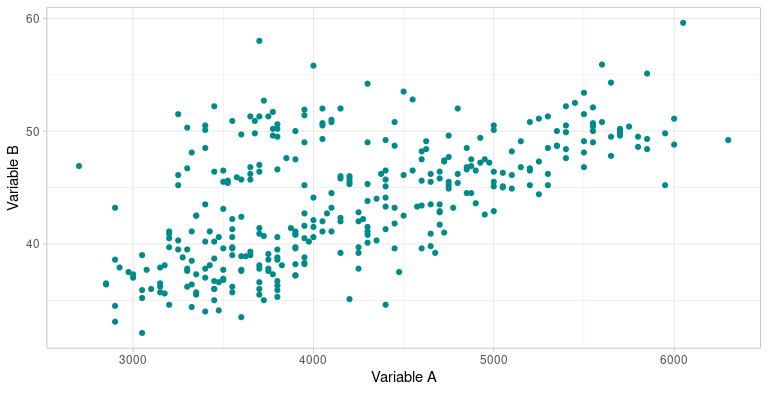
\includegraphics[width=\textwidth,keepaspectratio]{img/exemple_2D.png}

\end{frame}


\begin{frame}{Exemple en 2D}

Espace de départ + Les axes de l'espace d'arrivée

\centering
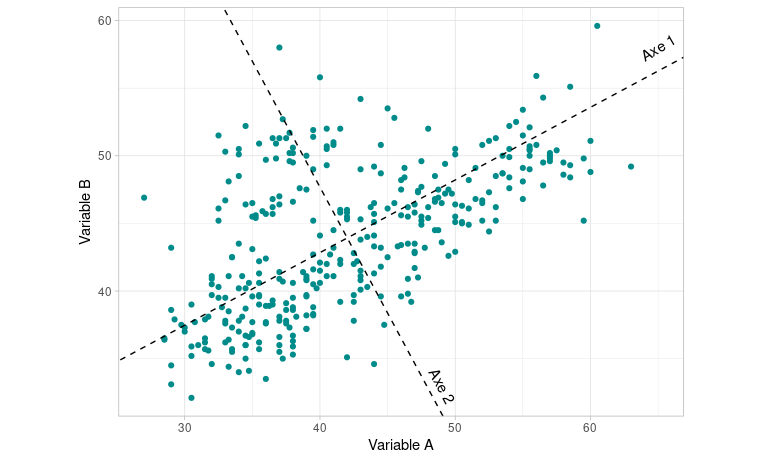
\includegraphics[width=\textwidth,keepaspectratio]{img/exemple_2D_axes.png}

\end{frame}


\begin{frame}{Exemple en 2D}

Espace d'arrivée 

\centering
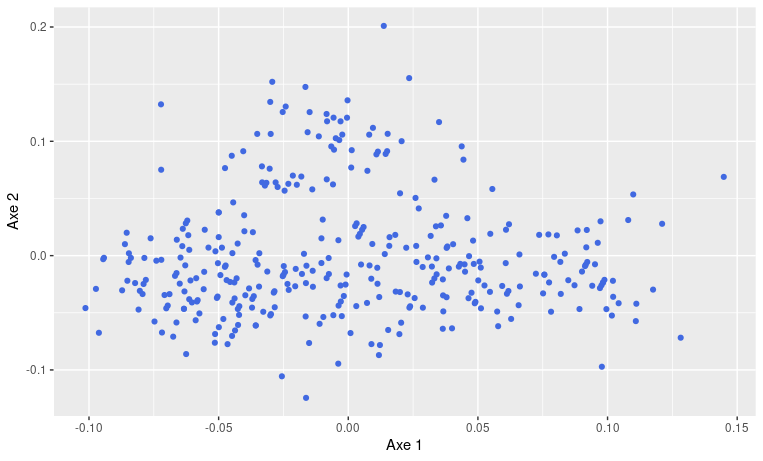
\includegraphics[width=\textwidth,keepaspectratio]{img/exemple_2D_arrivee.png}

\end{frame}


\begin{frame}{Exemple en 2D}

Espace d'arrivée + les axes de l'espace de départ

\centering
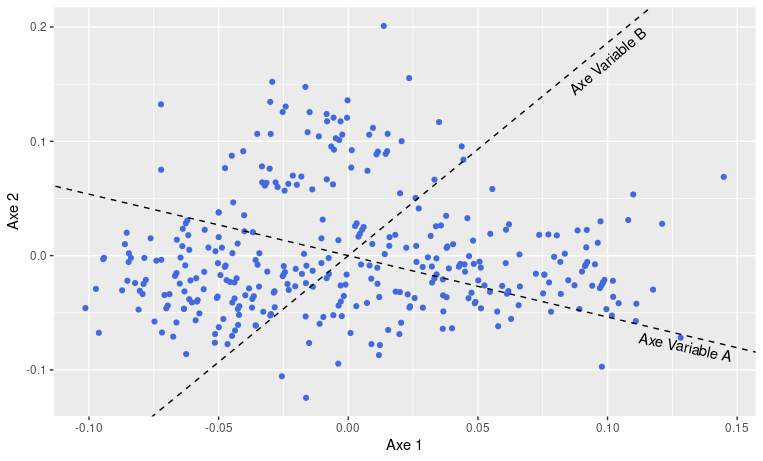
\includegraphics[width=\textwidth,keepaspectratio]{img/exemple_2D_arrivee_axes.png}

\end{frame}




\begin{frame}


espace de départ $\rightarrow$ ACP $\rightarrow$ espace d'arrivée 

\end{frame}




\begin{frame}{Calcul des axes}

Les \alert{axes} sont les \alert{vecteurs propres} de la matrice de corrélation de $P$, $Cor_P$. 
On peut les calculer (ouf !)

\medskip

l'ACP est le calcul d’une transformation linéaire qui \alert{re-projette} des vecteurs-individus dans un nouvel \alert{espace} -- l'espace d'arrivée--  constitué par les \alert{nouveaux axes}.

\medskip

On appelle ces axes \alert{composantes}, elles sont \alert{linéairement indépendantes} et forment une \alert{base} de l'espace d'arrivée.
\end{frame}



\begin{frame}{Nombres de composantes et inertie}

L'ACP capture l'inertie de $P$ en créant des composantes (les vecteurs propres de  $Cor_P$). 

\medskip

Il y a autant de composantes possibles que de dimensions de l'espace de départ. 

\medskip  


L'intérêt de l'ACP est de pouvoir se limiter à \alert{quelques} composantes  pour à la fois 
\begin{itemize}
\item  capturer suffisamment l'inertie ($\approx$ l'information) de $P$
\item  réduire la dimensionnalité ($\approx$ complexité) de $P$
\end{itemize}

\end{frame}


\begin{frame}{Nombres de composantes et inertie}


L'inertie capturée par une composante $k$ est sa valeur propre , $\lambda_k$

On ordonne les composantes par valeur propre décroissantes:

La 1\textsuperscript{ère} composante correspond au vecteur propre de plus grande valeur propre, elle capture la plus grande proportion d'inertie

La 2\textsuperscript{nde} composante correspond au  vecteur propre de la seconde plus grande valeur propre , elle capture la seconde plus grande proportion d'inertie 

\medskip

et ainsi de suite.

\medskip


Si les variables sont centrées et réduites, leur somme vaut $Dim(P)$ 


\end{frame}




\section{Interpréter les résultats d'une ACP}


\begin{frame}{Les objets à explorer dans les résultats d'une ACP}


\begin{itemize}
  \item \alert{Dimensionnalité} : L'essentiel de l'inertie est-elle exprimée en peu de dimensions dans l'espace d'arrivée ? 
  \item \alert{Colinéarité des variables} : Comment les variables de l'espace de départ sont-elles corrélées entre elles et aux axes de l'espace d'arrivée ? 
  \item \alert{Contribution} : À quel point Individus et Variables  contribuent aux axes de l'espace d'arrivée ?
  \item \alert{Représentation} : Les Individus et Variables sont ils·elles bien représenté·e·s  par les axes de l'espace d'arrivée ?

\end{itemize}



\end{frame}





\begin{frame}{Dimensionnalité : Nombres de composantes et inertie}


Le \alert{scree plot} montre la proportion d'inertie capturée par les différentes composantes. 
La valeur propre associée aux vecteurs propres (axes) est proportionnelle à l'inertie capturée.

\centering
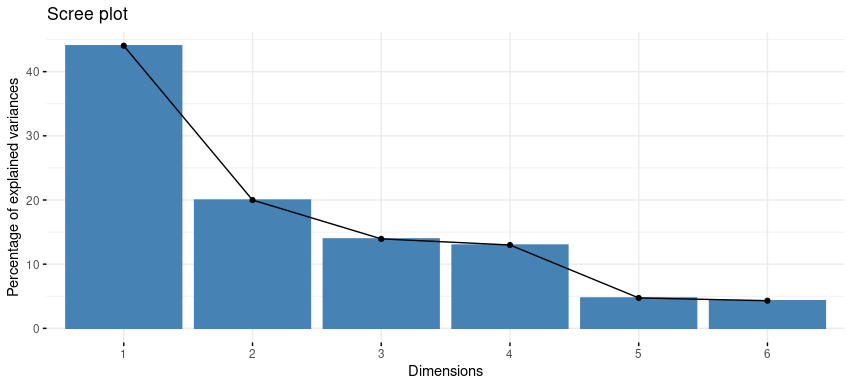
\includegraphics[width=\textwidth,keepaspectratio]{img/scree_plot.png}



\end{frame}



\begin{frame}{Dimensionnalité : Nombres de composantes et inertie}


\alert{Idéalement}, les premières (2 ou 3 ) composantes capturent une partie significative (e.g. $\gtrapprox50\%$ de l'inertie de $P$


\medskip


Cela signifie que les composantes \alert{résument bien} l'information contenue dans les variables de $P$, en \alert{peu de dimensions}.

\end{frame}




\begin{frame}{Dimensionnalité : Nombres de composantes}


Pour profiter du "résumé" de l'ACP , il faut se limiter à un certain nombre de composantes pour définir l'espace d'arrivée dans lequel on reconstituera les individus et variables. 

\medskip

Heuristiques du choix du nombre: 

\begin{itemize}
  \item On garde les $q$ axes que l'on sait \alert{interpréter} : 2 ou 3 !
  \item "coude" dans le scree-plot.
  \item ne conserver que les $\lambda > 1$ ou $\lambda > 2$
  \item Karlis-Saporta-Spinaki :  conserver les $\lambda$ t.q. $\lambda > 1 + 2 \sqrt{\frac{p-1}{n-1}}$
  \item Gavish \& Donoho (2014) : $\lambda = \frac{4 \sigma \sqrt{n}}{\sqrt{3}}$ avec $\sigma$ le bruit estimé dans les données.
  \end{itemize}

\begin{tiny}
Avec $\lambda$, les valeurs propres associées aux axes, $p$ le nombre de variable de $P$, et $n$ la taille de $P$
\end{tiny}


\end{frame}







\begin{frame}{Nombres de composantes et visualisation}


En pratique , si on sélectionne $q$ composantes, il faudra projeter les individus et les variables dans $C_q^2$ plans pour les visualiser.

\medskip

Si $q=3$, il faut 3 graphiques  $\{(q_1,q2) , (q_2,q_3), (q_1,q_3)\} $.

Si $q=4$, il en faut 6 !

\end{frame}





\begin{frame}{L'espace d'arrivée}

On sait passer de l'espace de départ à l'espace d'arrivée : 
On peut \alert{projeter} les variables et les individus dans l'espace d'arrivée

\medskip

De cette projection on tire beaucoup d'information utiles: 


\begin{itemize}
\item corrélations de variables
\item contribution / représentation  des variables 
\item contribution / représentation des individus 
\item regroupements d'individus
\end{itemize}
\end{frame}



\section{Projection des variables}



\begin{frame}{Colinéarité des variables}

Rappel : les variables sont des vecteurs dans l'espace des individus. 

On peut projeter les variables dans l'espace d'arrivée : 

\begin{center}
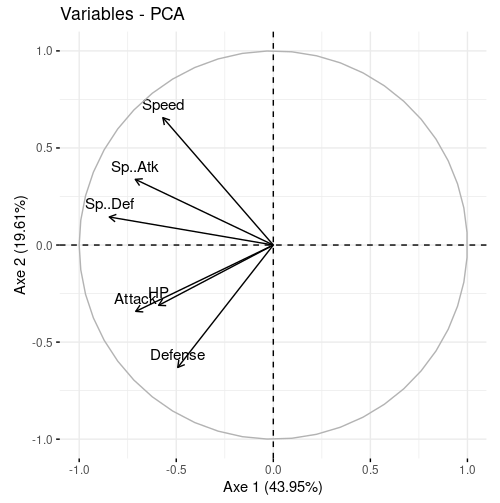
\includegraphics[width=0.45\textwidth,keepaspectratio]{img/cercle_trigo_ACP_var.png}
\end{center}
\begin{spacing}{0.7}
\begin{small}
Si les variables sont centrées et réduites lors de l'ACP, on peut les représenter dans un cercle de corrélation et évaluer visuellement leur  corrélation
\end{small}
\end{spacing}

\end{frame}


\begin{frame}{Colinéarité des variables}

\begin{center}
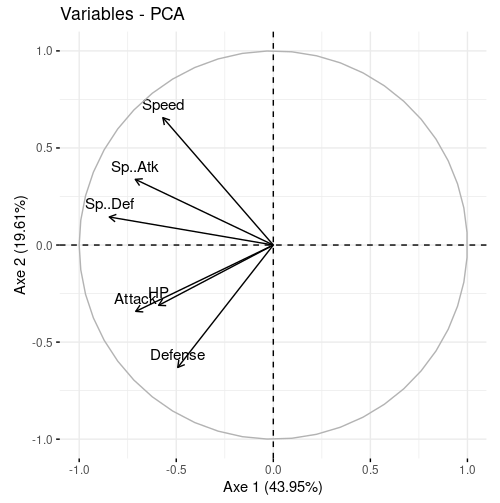
\includegraphics[width=0.5\textwidth,keepaspectratio]{img/cercle_trigo_ACP_var.png}
\end{center}

\begin{spacing}{0.7}
Variable $\leftrightarrow$  Flèche 

Coordonnées de la variable $\leftrightarrow$ \alert{corrélation linéaire}  avec les composantes

Proximité au cercle $\leftrightarrow$ qualité de \alert{représentation} de la variable

Angle des variables $\leftrightarrow$ corrélation des variables entre elles
\end{spacing}



\end{frame}



\begin{frame}{Colinéarité des variables}

\begin{center}
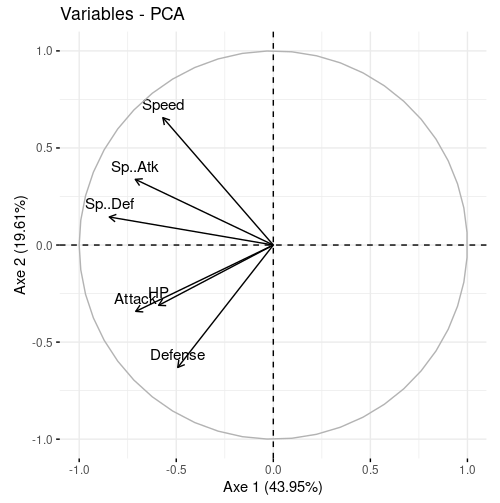
\includegraphics[width=0.5\textwidth,keepaspectratio]{img/cercle_trigo_ACP_var.png}
\end{center}


\begin{itemize}
\item la corrélation de \texttt{Defense} avec l'Axe 1 est de -0.5
\item \texttt{Attack} et \texttt{HP} sont très corrélées
\item \texttt{Speed} et \texttt{Defense} sont (linéairement) indépendantes
\end{itemize}



Ici : regroupement de variables ? Oui ! 


\end{frame}




\begin{frame}{Contribution des variables}

La \alert{contribution} d'une  variable $v$ à l'inertie de l'axe $k$  est la coordonnée carrée  de $v$ sur l'axe $k$ divisée par son inertie.

$$ ctrb_{vk} =\frac{c_{vk}^2}{\lambda_k} $$ 


Plus la contribution d'une variable est élevée , plus elle est importante pour expliquer la variabilité de $P$


\end{frame}


\begin{frame}{Qualité de représentation des variables}

La \alert{qualité de représentation} d'une  variable $v$ par l'axe $k$  est la coordonnée carrée  de $v$ sur l'axe $k$ :

$$ctrb_{vk} = c_{vk}^2$$ 

\end{frame}



\section{Projection des individus}


\begin{frame}{Nuage de points des individus dans le plan}

Rappel : les individus sont des vecteurs dans l'espace des variables de $P$. 

On peut projeter les individus dans l'espace d'arrivée : 

\begin{center}
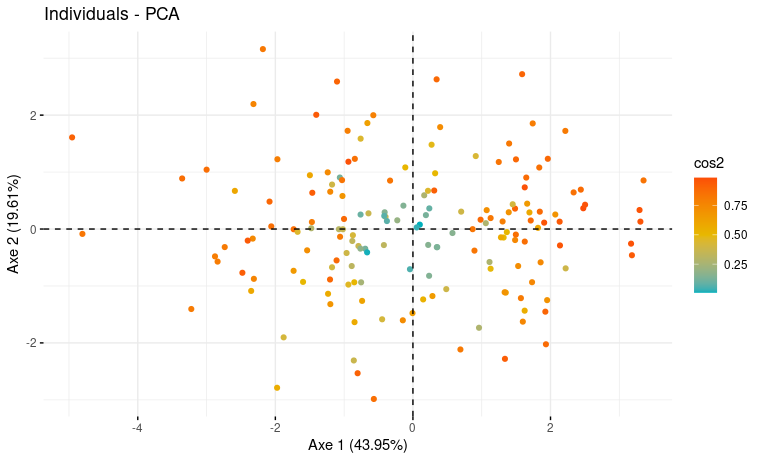
\includegraphics[width=0.65\textwidth,keepaspectratio]{img/cercle_trigo_ACP_ind.png}
\end{center}
\begin{spacing}{0.7}
Parfois cela fait apparaitre des regroupements (ici, pas vraiment) 
\end{spacing}

\end{frame}






\begin{frame}{Bilan de l'ACP}


  \begin{columns}[T,onlytextwidth]
    \column{0.48\textwidth}
        \begin{alertblock}{Avantages}
        	\begin{itemize}
        		\item Réduit la dimensionnalité
        		\item Regroupe les variables et les individus 
        	\end{itemize}
      	\end{alertblock}

    \column{0.48\textwidth}
	\metroset{block=fill}
    
      \begin{block}{Limites}
        \begin{itemize}
            \item Composantes difficiles à interpréter en elles-mêmes
            \item Que faire si $p$ est grand et si les premières composantes capturent peu d'inertie ?
          \end{itemize}
      \end{block}

      
  \end{columns}
\end{frame}




\begin{frame}{Pokémonologie}


\begin{columns}[T,onlytextwidth]
    \column{0.35\textwidth}

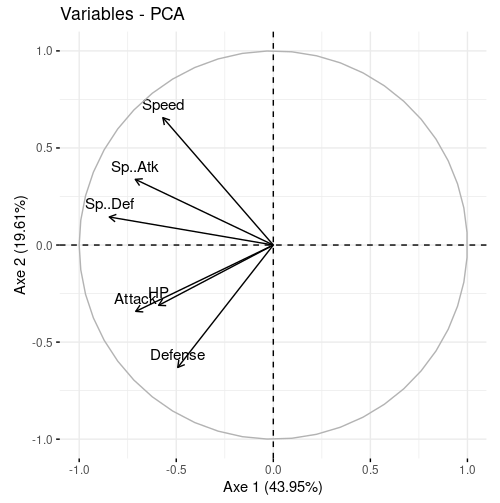
\includegraphics[width=\textwidth,keepaspectratio]{img/cercle_trigo_ACP_var.png}


  \column{0.65\textwidth}
\begin{small}  
\begin{itemize}
\item L'Axe 1 "prend tout" : c'est la puissance générale des pokémon, une sorte de \alert{score global}
\item L'Axe 2 sépare les variables en \alert{deux groupes} : celle du  combat "standard" (\texttt{Attack, Defense,HP}) et celles du combat "spécial/rapide" (\texttt{Sp..Atk, SP..Def, Speed})
\item On pourrait être tenté de diviser les pokemons en "Costauds classiques " vs. "Ninjas spéciaux" . 
\end{itemize}
\end{small}

\end{columns}

\medskip  
\medskip  \medskip  \medskip  \medskip  
\begin{tiny}
Merci à Anh Le , \url{https://anhqle.github.io/gotta-plot-them-all/}
\end{tiny}


\end{frame}




\begin{frame}{Ressources utiles}


\url{http://www.sthda.com/french/articles/38-methodes-des-composantes-principales-dans-r-guide-pratique/73-acp-analyse-en-composantes-principales-avec-r-l-essentiel}

\end{frame}


\begin{frame}{Animation}
  \begin{itemize}[<+- | alert@+>]
    \item \alert<4>{This is\only<4>{ really} important}
    \item Now this
    \item And now this
  \end{itemize}
\end{frame}



\begin{frame}[standout]
Mono message sur une diapo
\end{frame}


\begin{frame}{Formules}
  \begin{equation*}
    A = \sum_{i=1}^{n} \left(1 + \frac{1}{x_i}\right)^{\alpha}
  \end{equation*}
\end{frame}


\end{document}